Shortbus \ref{fig:Shortbusfenster} ist ein Programm (Desktopanwendung) welches in der seriellen- aber auch Netzwerkkommunikation zum Einsatz kommt. 
Es handelt sich bei Shortbus um ein Modbus RTU und Modbus TCP/IP Scanner.
Dabei ist die Hauptaufgabe bei der seriellen Kommunikation das Auslesen und Einschreiben von Werten in das Modbus Register welcher einer Client/Server Architektur folgt.
Das Programm unterstützt neben dem Auslesen und Einschreiben von Werten in Modbus Register auch das  automatische Einschreiben in ein Modbus Register (Zweck: automatische Testung einer Client/Server Verbindung)
Shortbus unterstützt noch andere Funktionen (Netzwerkfunktionen), doch diese sind in der seriellen Kommunikation nicht relevant. 
\cite[vgl.][]{software.informer:2024}

\begin{figure}[H]
	\centering
	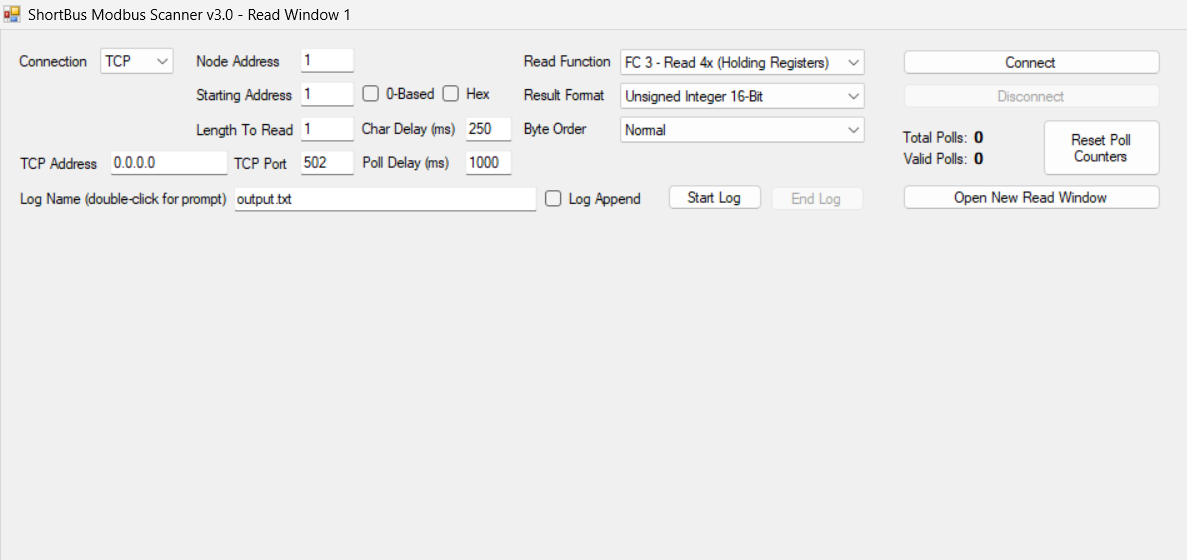
\includegraphics[width=1\linewidth]{Bilder/shortbus_fenster}
	\caption{Shortbus Desktopanwendung (ohne Inputs)} 
	\label{fig:Shortbusfenster}
\end{figure}

\subsection{Shortbus allgemeiner Teil}
Shortbus lässt sich in 2 große Bereiche gliedern. Das komplette Anzeigefenster kann in den oberen Teil siehe Abb.~\ref{fig:Shortbuseingabe} und einen unteren Teil Abb.~\ref{fig:Shortbusausgabe} aufgeteilt werden.
Im oberen Teil von Shortbus Abb.~\ref{fig:Shortbuseingabe} erfolgen die gesamten Eingaben was das System (Client/Server) betrifft:
\begin{itemize}
	\item Connection: Das ist die Art wie man sich mit dem System verbinden möchte. Man unterscheidet hierbei meist zwischen TCP (Transmission Control Protocol) oder COM (Schnittstelle am Laptop meist COM7)
	
	\item Node Adresse: Ist die Adresse, welche vom Bauteil verwendet wird. Jedes Bauteil (\zB \gls{qbm}  oder EBM-Papst) hat eine eigene Node Adresse.
	
	\item Starting Address: Diese bestimmt das erste Register was Ausgelesen werden soll. Die Register und deren Adressen können wie folgt angegeben werden:
		\begin{itemize}
			\item ob das Register bei null anfängt (0-Based) oder nicht
			\item wie das Register angegeben ist Hexadezimal (Hex) angegeben wird oder nicht
		\end{itemize}
	\item Length To Read: Gibt an wie viele Register ausgelesen werden. 
	\item Read Function: Hier wird die Registerart angegeben.
\end{itemize}

Im unteren Teil Abb.~\ref{fig:Shortbusausgabe} erfolgt die Ausgabe der einzelnen Modbus Register.  


  

\subsection{Shortbus Anwendung in der Entwicklungs- \ac{rltanlage}}

In der Entwicklungs- \ac{rltanlage} wird die Schnittstelle COM7 (USB-Port des Laptops) verwendet um eine Kommunikation (Connection) mit dem Modbus aufzubauen. Dabei wird der Modbus per Kabel  Abb.~\ref{fig:modbus_usbkabel} erweitert und auf der einen Seite mit dem Laptop und dessen USB-Schnittstelle verbunden. Die andere Seite wird in der \acp{rltanlage} auf den bestehenden Modbus angeschlossen. 

\begin{figure}[H]
	\centering
	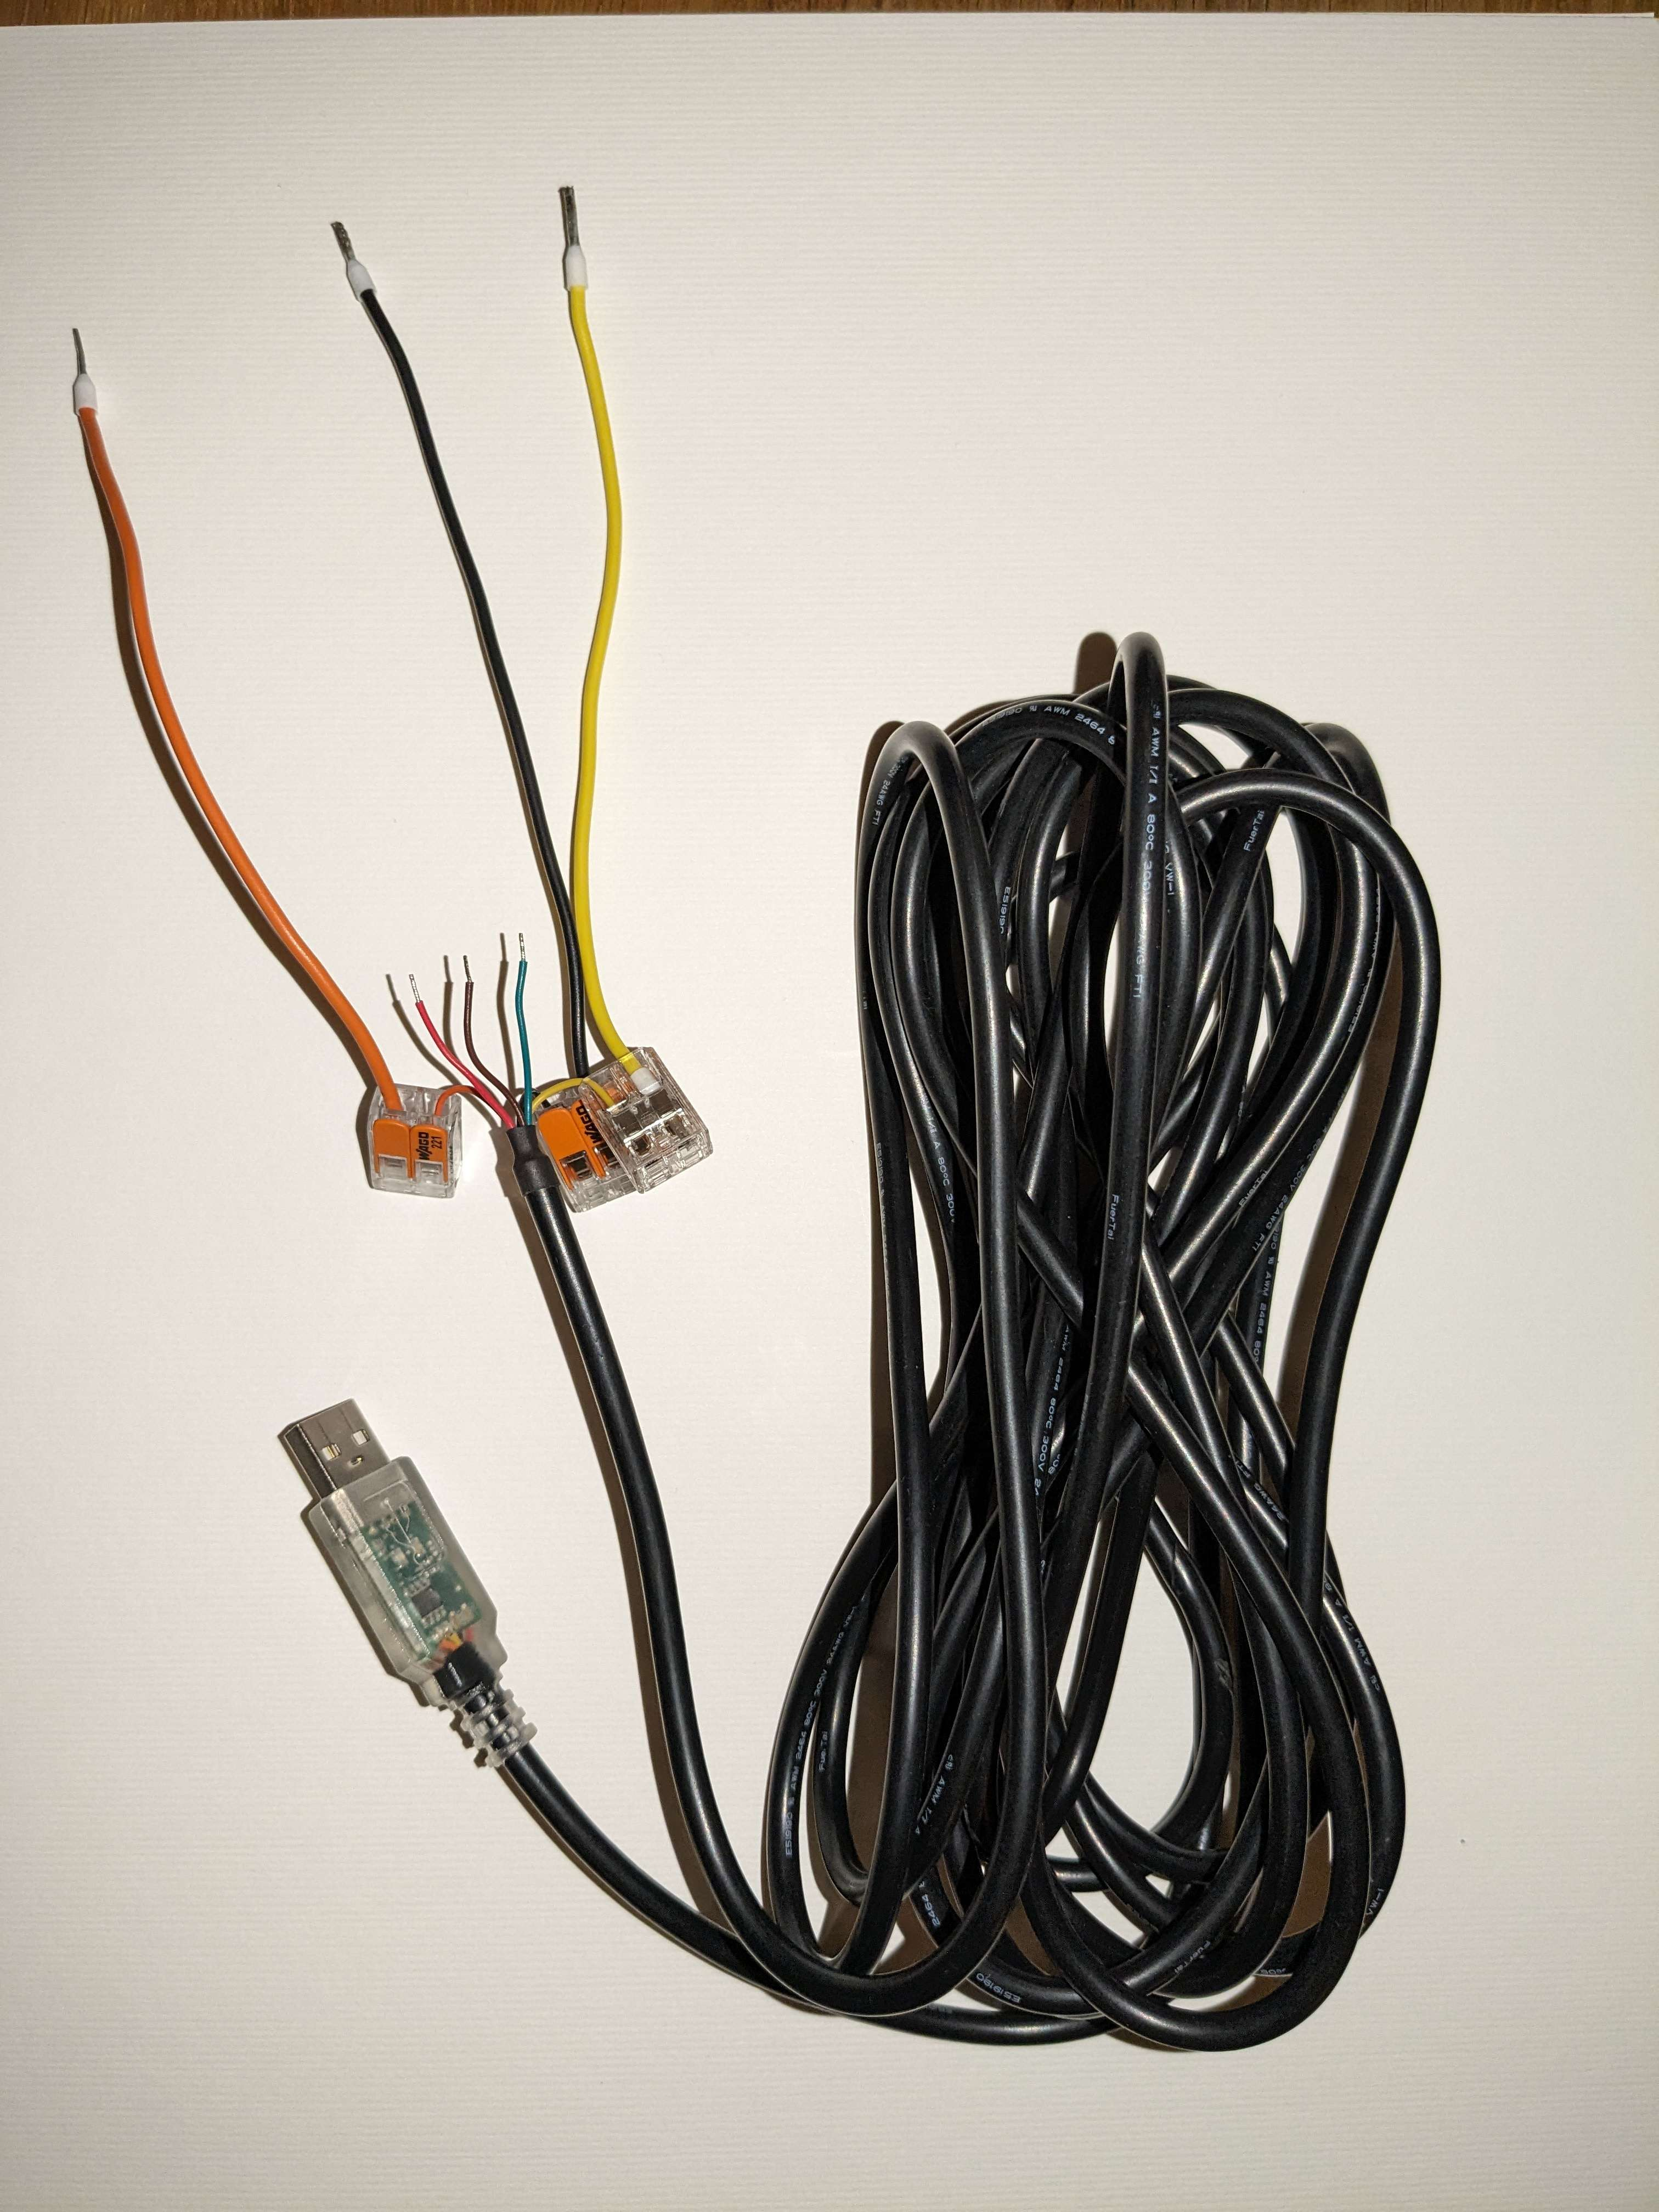
\includegraphics[width=0.3\linewidth]{Bilder/modbus_usbkabel}
	\caption{Modbus USB-Kabel} 
	\label{fig:modbus_usbkabel}
\end{figure}

Danach werden die Einzelnen Komponenten der seriellen Kommunikation angegeben (oberer Teil des Shortbus Fensters) Abb.~\ref{fig:Shortbusausgabe}:
\begin{itemize}
	\item Baudrate (9600)
	\item Parity (Even)
	\item Stop Bits (1)
	\item Node Adresse (2)
	\item Starting Address 1 (Register fängt bei eins an und ist in nicht in Hexadezimal angegeben)
	\item Length To Read (Die ersten 85 Werte sollen ausgegeben werden)
	\item Read Funktion (FC 3 - Holding Register)
\end{itemize}

Beschreibung der Werte und Funktion von: Baudrate, Parity, Stop Bits, Read Funktion siehe Kapitel\ref{modbus_funktionsweise}.
Im Projekt wurde zudem die Funktion Write Multiple verwendet Abb.~\ref{fig:writemultiple}. Diese Funktion wurde eingesetzt um zu Testen ob das passende Register für \zB die Ventilatoren, ausgelesen wurde. Dabei wurde in das Register ein Wert eingeschrieben und getestet ob die Ventilatoren auf das Verändern des Sollwertes reagieren.

\begin{figure}[H]
	\centering
	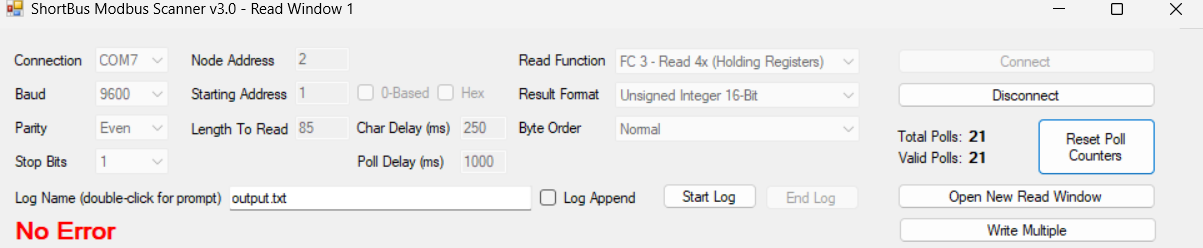
\includegraphics[width=1\linewidth]{Bilder/shortbus_eingabe}
	\caption{Shortbus Eingabefenster} 
	\label{fig:Shortbuseingabe}
\end{figure}


\begin{figure}[H]
	\centering
	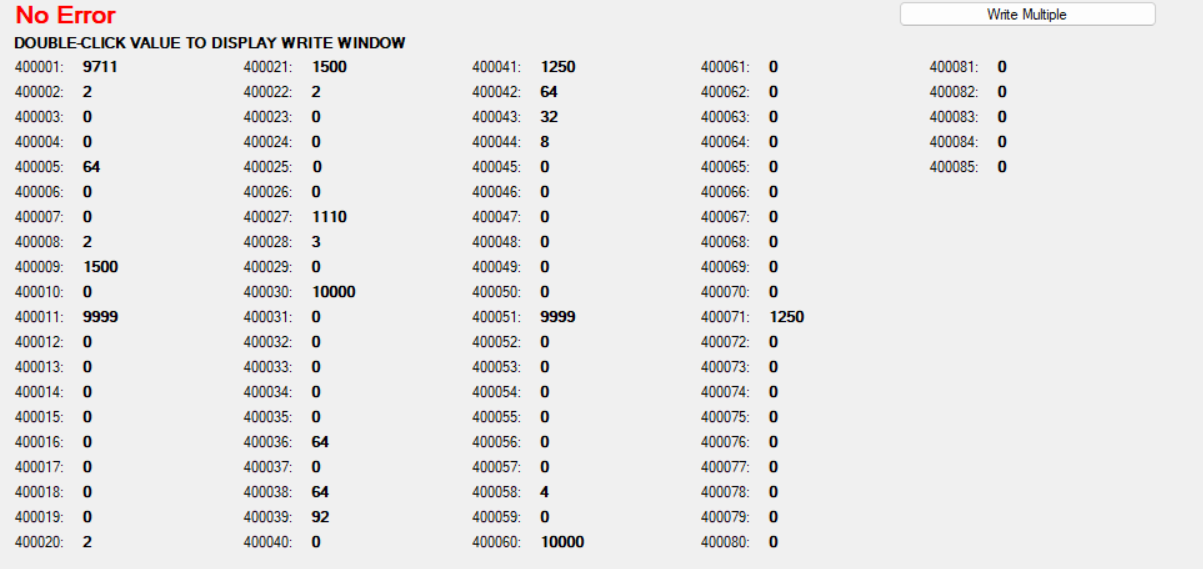
\includegraphics[width=1\linewidth]{Bilder/shortbus_ausgabe}
	\caption{Shortbus Ausgabefenster} 
	\label{fig:Shortbusausgabe}
\end{figure}

\begin{figure}[H]
	\centering
	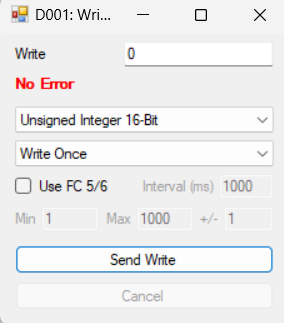
\includegraphics[width=0.3\linewidth]{Bilder/write_multiple_fenster}
	\caption{Shortbus Write Multiple Fenster} 
	\label{fig:writemultiple}
\end{figure}

\subsection{Shortbus Registerauslesung}

In der \ac{rltanlage} wurden mehrere \gls{qbm} von Siemens eingebaut. Aufgabe war es bei diesen und allen andern Bauteilen welche in der \ac{rltanlage} verbaut waren, die Register zu den einzelnen Werten herauszufinden um diese später in den Konfigurations-Files und für die Berechnungen bereitzustellen. 

Die ersten Versuche siehe Kapitel \ref{ersteauslesung}, etwas auszulesen wurden durch einen einfachen Aufbau von einem oder zwei \gls{qbm}  bewerkstelligt. Dabei wurden herausgefunden auf welchen Register der Druckunterschied angezeigt wird. Durch das anschließen von Temperatursensoren konnte man überprüfen ob auch die Register für die Analog Input Ports (Temperatur) auf die richtigen Register geschrieben worden waren.

\begin{figure}[H]
	\centering
	\includegraphics[angle=90,width=0.5\linewidth]{Bilder/erste_auslesung}
	\caption{Erste Werte Auslesen inkl. laufender Software} 
	\label{fig:ersteauslesung}
\end{figure}

Beschreibung der Auslesung anhand eines Beispiels Abb.~\ref{fig:Shortbusausgabe} (\gls{qbm}):
\begin{itemize}
	\item Bei Diesem \gls{qbm}  kommt auf dem ersten Register die genaue Typenbezeichnung des \gls{qbm} .  
	\item Auf dem Register 5 und 7 kommen die gemessenen Druckunterschieden (gemessen in Pascal(Pa)) herein. 
	\item Die Register 9 und 11 sind jeweils die zwei verbauten Analog Input Ports welche auch wiederum zwei Funktionen haben können:
	\begin{itemize}
		\item 1. Variante: Es sind Temperatursensoren (\zB Nickel1000) angeschlossen (Ausgabe in °C)
		\item 1. Variante: Es sind Klappen (\zB WRG-Klappe) angeschlossen (Ausgabe in mV)
	\end{itemize}
	\item Auf dem Register 27 und 57 sind beim \gls{qbm} die Analog Output Ports zu finden
	
	\cite[vgl.][]{siemens:2021}
\end{itemize} 
 